\documentclass[10pt]{article}
\usepackage{parskip}
\usepackage[utf8]{inputenc}
\usepackage[left=2.00cm, right=2.00cm, top=2.00cm, bottom=2.00cm]{geometry}
\usepackage[spanish]{babel}
\usepackage{graphicx,subfig}
\usepackage{fancyhdr}
\usepackage{pgfplots}
\graphicspath{{Imagenes/}}
\usepackage{enumerate} 
\usepackage{multicol}
\usepackage{tabularx}
\usepackage{amssymb}
\usepackage{adjustbox}
\usepackage{amsmath}
\usepackage{cancel}
\begin{document}


\pagestyle{fancy}
\cfoot{}


%Cabeceras
\rhead{Movimiento ondulatorio en una cuerda I, II.}
\lhead{}

%Portada
\begin{titlepage}
	\newgeometry{
		left=25mm,
		right=25mm,
		top=5mm,
		bottom=30mm,
		headheight = 0 mm
	}

	\begin{figure}[t]
		\subfloat{
\includegraphics[width=0.15\textwidth]{Logo_IPN}}
		\hspace{0.6\textwidth}
		\subfloat{
\includegraphics[width=0.22\textwidth]{LogoEsime}}
	\end{figure}

	\centering
	{\bfseries\Huge Instituto Politécnico Nacional. \par}
	\vspace{1cm}
	{\scshape\Large Ingeniería en Comunicaciones y Electrónica. \par}
	\vspace{0.3cm}
	{\scshape\Large Laboratorio de Ondas Mecanicas.  \par}
	\vspace{1cm}
	{\scshape\Huge Como en el temblor?! \par}
	\vspace{1cm}
	{\itshape\Large Movimiento ondulatorio en una cuerda I, II. \par}
	{\Large 3CM1\par}
	\vfill
	
	\vfill
	{\Large Noviembre 2023. \par}

\end{titlepage}

\tableofcontents
\newpage
\begin{center}
	Hernández Huerta Jose Emilio, 
	Hernández Sanluis Danna Estefany,  
	Garduño Bejarano Nataly,
	Mojica Reyes Rogelio,
	Morlan Juárez Bruno Tonatiuh,  
	Santos Marañón María Renée.
\end{center}

\section{Resumen.}

Se realizaron un par de experimentos relacionados a la velocidad de propagación de una onda mecánica, generada por un motor de 220 V (con reductor de velocidad 1:10) y un medio elástico (cuerda de goma). 
\begin{multicols}{2}

\section{Objetivo.}
El objetivo general de esta practica de laboratorio es estudiar y comprender el comportamiento de un sistema que involucra el generador de una onda mecánica y un medio elástico, para determinar la velocidad de propagación con todas sus correspondientes componentes mediante el uso de experimentos controlados y análisis de datos.


\section{Introducción.}
El estudio del movimiento ondulatorio es fundamental en la comprensión de diversos fenómenos naturales y aplicaciones tecnológicas. En este trabajo, nos enfocamos en el análisis del movimiento ondulatorio en una cuerda, explorando aspectos relacionados con la velocidad de propagación, la frecuencia y la longitud de onda.



\section{Marco teórico.}

\subsection{Onda Transversal}
Las ondas transversales son un tipo de onda en la que la perturbación se propaga perpendicularmente a la dirección de la energía transportada por la onda. Algunos ejemplos comunes de ondas transversales son las ondas electromagnéticas (como la luz) y las ondas sísmicas secundarias (ondas S) en geofísica.
En una onda transversal, las partículas del medio oscilan perpendicularmente a la dirección de la propagación de la onda. Esto contrasta con las ondas longitudinales, donde las partículas oscilan en la misma dirección de la propagación de la onda. Un ejemplo visual de una onda transversal es una onda en una cuerda cuando la cuerda se agita verticalmente, y la onda viaja horizontalmente.
En el caso de ondas electromagnéticas, como la luz, el campo eléctrico y el campo magnético oscilan perpendicularmente entre sí y en la dirección de propagación. Este tipo de ondas juega un papel crucial en diversas áreas, desde la óptica hasta las comunicaciones inalámbricas.
En resumen, en las ondas transversales, la perturbación se desplaza de manera perpendicular a la dirección de propagación, lo que las distingue de las ondas longitudinales, donde la perturbación se desplaza en la misma dirección de la propagación.
\subsection{Rapidez de una onda Transversal}
La rapidez de propagación de una onda es una propiedad fundamental que describe cómo la perturbación o la energía asociada con la onda se mueve a través de un medio. Ya sea en forma de ondas sonoras que atraviesan el aire, ondas en una cuerda vibrante, o incluso ondas electromagnéticas como la luz, la velocidad a la cual estas perturbaciones se desplazan es esencial para comprender y caracterizar los fenómenos ondulatorios.
La rapidez de propagación de una onda está estrechamente relacionada con la frecuencia y la longitud de onda de la onda misma. Diferentes tipos de ondas tienen diferentes velocidades características en un medio dado. Por ejemplo, las ondas sonoras viajan a través del aire a una velocidad específica, mientras que las ondas en una cuerda o las ondas electromagnéticas tienen velocidades características en sus respectivos medios.
Esta propiedad no solo es central para la teoría de las ondas, sino que también tiene aplicaciones prácticas en diversas disciplinas. Comprender la velocidad de propagación de las ondas es esencial en campos como la acústica, la ingeniería de telecomunicaciones, la geofísica y la óptica. En esta introducción, exploraremos los conceptos clave relacionados con la rapidez de propagación de las ondas y su importancia en la comprensión de fenómenos naturales y tecnológicos.



\section{Experimento 1.- Determinación de la velocidad de fase}
\subsection{Desarrollo - Cuerda de hule o goma}
Realizamos este experimento, montando en sistema como se nos dejó indicado en el manual de laboratorio, en esta parte no existe ningún tipo de problema ya que el profesor y el equipo de técnicos montaron en motor, con la cuerda combinada.

Lo que nos pidió el manual fue presentar dos antinodos en una imagen, y después de manipular el generador de onda a cierta frecuencia, pudimos llegar a notar ciertas características de una onda transversal. (Imagen 1) \\

\begin{center}
	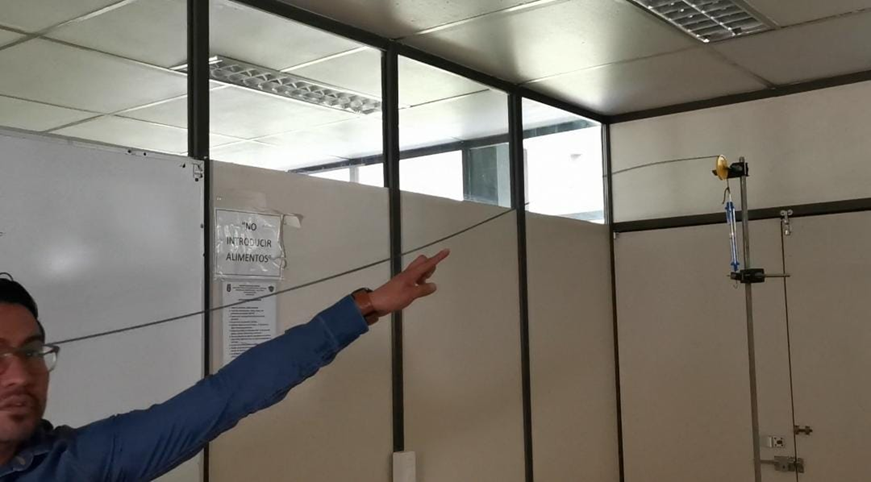
\includegraphics[width=5.05cm,height=3.06cm]{Imagenes/4.png}
	\captionof{figure}{Imagen donde se observan algunos de los nodos generados por el motor.}
	\label{fig:1}
\end{center}
Para la determinación de la rapidez de propagación de una onda transversal, usamos unos datos proporcionados por nuestro profesor, en los cuales usamos lo que nosotros conocíamos como efecto concierto (ecuación de rapidez de propagación de una onda), la cual involucraba la longitud de onda y la frecuencia de la ya antes menciona, lo que nos llevó a una serie de resultados que nos parecieron sensatos.
A continuación monstamos los resultados de esta parte del experimento:

Ecuaciones utilizadas\\
$L=n\frac{\lambda}{2}$...$\lambda=\frac{2L}{n}$\\
L=2.60m\\
m=0.10gr\\
$\lambda=\frac{2(1.25)}{3}$=0.833m V=10.91 m/s \\
------------------------------------------------------\\

n=2 d=0.92m f=17.1Hz A=2.25cm\\
$\lambda=\frac{2(0.92)}{2}=0.92$ $ V=15.732m/s$\\
------------------------------------------------------\\
n=2 d=0.78 f=17Hz A=2.5\\
$\lambda=\frac{2(2.78)}{2}=0.78$ $V=13.26m/s$\\
------------------------------------------------------\\
\subsection{Desarrollo - Cuerda de algodón}
En esta segunda parte solo hicimos un cambio en el sistema, pero en esencia es el mismo procedimiento, y la misma meta a qué queríamos llegar (la obtención de la rapidez de una onda).
Pero en un medio muy diferente, ya que ahora ya no hablamos de un medio cien porciento elástico, sino de tiene un coeficiente de elasticidad escaso (no inexistente, pero no es la característica principal de este material). Y llegamos a los siguientes resultados:

n=3 d=0.67 f=21Hz A=1.25cm\\
$\lambda=\frac{2(0.67)}{3}=0.426$ $V=8.946$\\
------------------------------------------------------\\
n=3 d=0.60 f=23Hz A=3.5 cm
$\lambda=\frac{2(0.60)}{3}=0.4m $ $V=9.2 m/s$\\

\subsection{Segunda parte (cuerda de algodon)}
L=2.50m\\
m=0.20gr\\
n=2 d=0.84m f=13.3Hz A=1cm\\
$\lambda=\frac{2(0.84)}{2}=0.84m$ $V=11.72 $ \\
------------------------------------------------------\\
n=2 d=0.90m f=12.7Hz A=2.5cm
$\lambda=\frac{2(0.90)}{2}=0.90m$ $V=11.43 $\\
------------------------------------------------------   \\
n=3 d=0.86m f=12.3Hz A=3cm\\
$\lambda=\frac{2(0.86)}{3}=0.86$ $V=10.578 $\\



\section{Experimento 2.- Determinación de la velocidad de fase en función de la fuerza aplicada a la cuerda}
La realización del experimento fue realizada en grupo mostrando cada paso por nuestro profesor, que utilizando el equipo con la cuerda anclada en un extremo a la rueda con el motor anclado a una polea mientras que el otro extremo de la cuerda está en la punta de una varilla apoyada verticalmente tal como la imagen 2. 
 
\begin{center}
	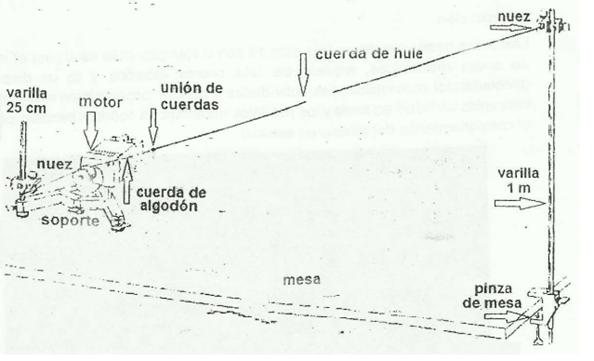
\includegraphics[width=5.05cm,height=3.06cm]{Imagenes/1.png}
	\captionof{figure}{Sistema del arreglo de la cuerda.}
	\label{fig:2}
\end{center}
Del sistema empleado, se midió la cuerda con el dinamómetro desde 0.5 N. Posterior a la medición de la cuerda, se activa el motor donde se encuentra la cuerda acanalada en el sentido de la menor fuerza midiendo la longitud de la onda creada por las oscilaciones de la rueda acanalada con un flexómetro. 
Para determinar la frecuencia del motor del movimiento de la cuerda se ocupó es estroboscopio iluminando la cuerda hasta que se vea congelada la imagen obteniendo lo de la imagen 3. 
\begin{center}
	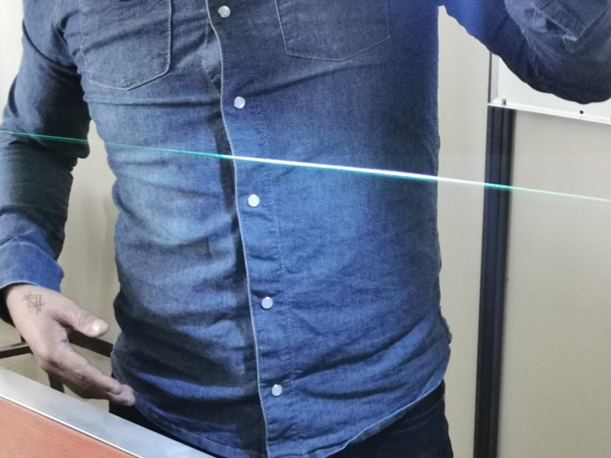
\includegraphics[width=5.05cm,height=3.06cm]{Imagenes/2.png}
	\captionof{figure}{Vista congelada de la onda vista por el estroboscopio
    generada por la cuerda y el motor en acción.}
	\label{fig:3}
\end{center}
En aumento de la velocidad del motor, se logran captar los antinodos reflejando una imagen clara de la onda. Imagen 4.
\begin{center}
	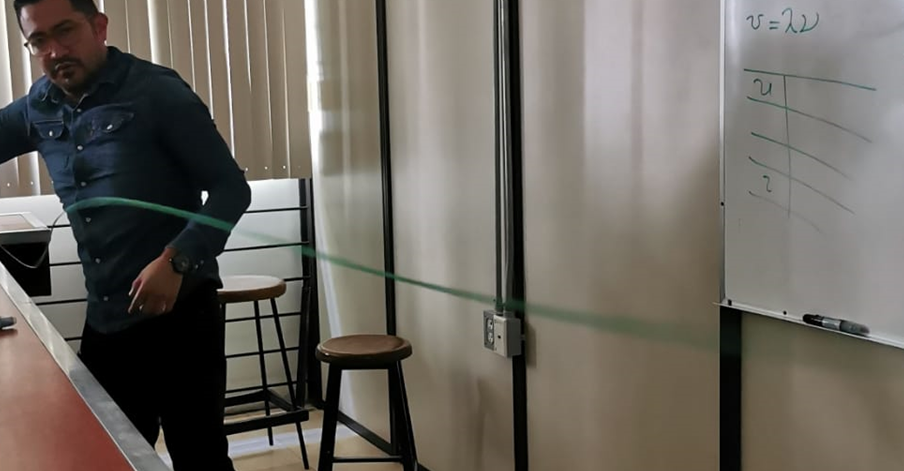
\includegraphics[width=5.05cm,height=3.06cm]{Imagenes/3.png}
	\captionof{figure}{Onda generada por el motor a alta potencia mostrando un nodo y antinodo.}
	\label{fig:4}
\end{center}

Tabulando la frecuencia vs la distancia se obtienen los siguientes datos usando el cambio de variable.
\begin{center}
    \begin{tabular}{|c|c|c|}
        \hline
        $F[N] \pm 0.05$ & $v[Hz] \pm 0.05$ & $\lambda[m] \pm 0.0005$ \\
        \hline
        0.50 & 9.60 & 1.7 \\
        1.00 & 12.20 & 1.9 \\
        1.50 & 14.60 & 1.9 \\
        2.00 & 15.40 & 2.1 \\
        2.50 & 16.00 & 2.3 \\
        3.00 & 16.50 & 2.4 \\
        3.50 & 17.40 & 2.5 \\
        4.00 & 19.60 & 2.3 \\
        4.50 & 21.60 & 2.3 \\
        5.00 & 22.80 & 2.2 \\
        \hline
    \end{tabular}\\
\textbf{Tabla 1}
\end{center}
    \
    Realizando el producto de la frecuencia y la distancia.
    \begin{center}
        \begin{tabular}{|c|c|}
        \hline
        $vf = \lambda f$ & $vf$ \\
        \hline
        $1.7 \times 0.50$ & 0.85 \\
        $1.9 \times 1.00$ & 1.9 \\
        $1.9 \times 1.50$ & 2.85 \\
        $2.1 \times 2.00$ & 4.2 \\
        $2.3 \times 2.50$ & 5.75 \\
        $2.4 \times 3.00$ & 5.4 \\
        $2.5 \times 3.50$ & 8.75 \\
        $2.3 \times 4.00$ & 9.2 \\
        $2.3 \times 4.50$ & 10.35 \\
        $2.2 \times 5.00$ & 11 \\
        \hline
    \end{tabular} \\
    \textbf{Tabla 2}
    \end{center}
    
Con base en la Tabla 2
\begin{center}
    \begin{tikzpicture}
        \begin{axis}[
            title={Gráfica 1},
            xlabel={$vf = \lambda f$},
            ylabel={$vf$},
            axis lines=left,
            xmin=0, xmax=12,  % Ajustar los valores máximos del eje x según tus datos
            ymin=0, ymax=12, % Ajustar los valores máximos del eje y según tus datos
            grid=both,
            legend pos=north west,  % Posición de la leyenda
            legend cell align={left}, % Alineación del texto en la leyenda
        ]
        
        % Puntos de datos
        \addplot [black, mark=*] coordinates {
            (0.85, 0.85)
            (1.9, 1.9)
            (2.85, 2.85)
            (4.2, 4.2)
            (5.75, 5.75)
            (7.2, 5.4)
            (8.75, 8.75)
            (9.2, 9.2)
            (10.35, 10.35)
            (11, 11)
        };
        
        % Leyenda
        \end{axis}
    \end{tikzpicture}
\end{center}



\subsection{Conclusión}
¿Qué significado tiene la cantidad que relaciona las variables y que se le proporciona la comparación con el cálculo de ($\lambda$) ($\upsilon$)?
El producto resultante de estas dos variables, representan la rapidez de una onda de propagación esto lo sabemos porque la longitud de onda y la frecuencia están estrechamente relacionadas. Al anterior teorema lo podemos explicar con el hecho de que la frecuencia de una onda representa la cantidad de oscilaciones o ciclos que la onda completa en un segundo, a medida que la frecuencia aumenta, la cantidad de ciclos por segundo aumenta. Por lo tanto, a medida que la longitud de onda disminuye, la distancia que la onda debe recorrer en cada ciclo también disminuye, y estos dos factores son lo que afecta la rapidez de propagación.

\section{Conclusiones.}
\subsection{Hernández Huerta Jose Emilio.}
Con esta practica podemos comprobar como se crean las ondas, analizamos sus formas y ademas hicimos comprovaciones para poder enalizar de una forma precisa las ondas generadas al igual que como cambian estas dependiendo del medio por el cual estas viajan.
\subsection{Hernández Sanluis Danna Estefany.}
\subsection{Nataly Bejarano Garduño.}
Es interesante ver el fenomeno causado por la cuerda y el movimiento ya que en cada una de las diferentes velocidades, ocurre una frecuencia diferente, y por lo tanto, una vista más amplia o corta de los nodos el movimiento de ondas en una cuerda es el medio por el cual se propaga energía de un punto a otro sin necesidad de transferir materia, mediante ondas mecanicas Un tipo de onda, y la que vimos en la practica, es la onda transversal. La cual es una onda en donde su perturbación es perpendicular a la dirección A su vez, notamos que la relación que existe entre un espacio recorrido igual a una longitud de onda y de tiempo empleado en recorrerlo, se le denota como velocidad de propagación.
\subsection{Mojica Reyes Rogelio.}
En resumen, a lo largo de estos experimentos, demostramos de manera convincente la velocidad de propagación con todas sus componentes por medio de un par de experimentos y mucho análisis. Al comprender la importancia de la relación que existía en la frecuencia y la longitud de una onda mecánica podemos concluir que estos son una parte fundamental del estudio y aplicación de muchas ramas de la ingeniería, la física y la matemática. 
\subsection*{Morlan Juárez Bruno Tonatiuh.}
Durante la realización de este experimento de forma muy rápida fue una buena manera de ver como se ven en forma física las ondas senoidales, conociendo de manera visual las características ya estudiadas en horario de clase, por lo que, es importante enforcarnos en los conceptos, esencialmente en los matemáticos para poder estudiarlas de manera correcta y precisa. 
\subsection*{Santos Marañón María Renée.}
En esta práctica aprendimos que el movimiento ondulatorio es un proceso de propagación de la energía mediante perturbaciones del medio donde se propaga, y sin trasferencia de materia. El movimiento ondulatorio trasporta energía y cantidad de movimiento. Pudimos observar el efecto Doppler que es el aparente cambio de frecuencia de una onda producida por el movimiento relativo de la fuente respecto a su observador. Y también cómo se quedaba congelada la imagen de la cuerda para poder realizar nuestras mediciones y tener cálculos más precisos. En una onda transversal a lo largo de una cuerda tensa, por ejemplo, la velocidad depende de la tensión de la cuerda y de su densidad lineal o masa por unidad de longitud. La velocidad puede duplicarse cuadruplicando la tensión, o reducirse a la mitad cuadruplicando la densidad lineal. SI tenemos una cuerda con una tensión y luego la sometemos a una perturbación se generan ondas y mientras mayor sea esta perturbación generaremos más ondas en todo lo largo de la cuerda que serán de la misma longitud cada una.

\subsection*{Uriel Grimaldi Díaz.}
\begin{thebibliography}{0}
    \bibitem{bragado}[Bragado, I. M. (2003). \textit{Física General.}]
    \bibitem{benchimol}[Benchimol, D. (c. 2020). \textit{Electrónica práctica.} USERSHOP.]
    \bibitem{peaktech}[Peaktech. (2016). \textit{Manual de Usuario Peaktech 2005.}]
    \bibitem{french}[French, A. P. (1971). \textit{Vibrations and Waves.} CRC Press.]
    \bibitem{kittel}[Kittel, C., \& Kroemer, H. (1980). \textit{Thermal Physics.} W. H. Freeman.]
    \bibitem{strogatz}[Strogatz, S. H. (2018). \textit{Nonlinear Dynamics and Chaos.} CRC Press.]
\end{thebibliography}

\end{multicols}

\end{document}
